\documentclass[8pt]{beamer}
\usepackage[english]{babel}
\usepackage[OT4]{fontenc}
\usepackage[utf8]{inputenc}
\usepackage{multirow}
\usepackage{hyperref}
\usepackage{amsmath}
\usepackage{xfrac}
\usepackage{bm}
\usepackage{hyperref}
\usepackage{amsfonts}
\usepackage{amssymb}
\usepackage{graphicx}
\graphicspath{{Fig/}}
\usepackage{tikz}
\usetikzlibrary{shapes,arrows,patterns, positioning, calc,decorations.pathmorphing, fit, plotmarks}
\pgfdeclaredecoration{penciline}{initial}{
    \state{initial}[width=+\pgfdecoratedinputsegmentremainingdistance,
    auto corner on length=1mm,]{
        \pgfpathcurveto%
        {% From
            \pgfqpoint{\pgfdecoratedinputsegmentremainingdistance}
                      {\pgfdecorationsegmentamplitude}
        }
        {%  Control 1
        \pgfmathrand
        \pgfpointadd{\pgfqpoint{\pgfdecoratedinputsegmentremainingdistance}{0pt}}
                    {\pgfqpoint{-\pgfdecorationsegmentaspect
                     \pgfdecoratedinputsegmentremainingdistance}%
                               {\pgfmathresult\pgfdecorationsegmentamplitude}
                    }
        }
        {%TO 
        \pgfpointadd{\pgfpointdecoratedinputsegmentlast}{\pgfpoint{1pt}{1pt}}
        }
    }
    \state{final}{}
}
\definecolor{violet}{RGB}{55,54,112}
\definecolor{darkgreen}{RGB}{75,141,75}
\definecolor{redish}{RGB}{161,35,44}
\definecolor{blueish}{RGB}{8,8,90}
\tikzstyle{input} = [rectangle, draw, fill=blue!10,text width=1cm, text centered, rounded corners, minimum height=4em]
\tikzstyle{class} = [rectangle, draw,minimum width=2cm, text width=2.5cm, text centered, minimum height=2em]
\tikzstyle{className} = [rectangle,fill=black!5, draw,minimum width=2cm, text width=2.5cm, text centered, minimum height=2em]
\tikzstyle{comment} = [text=violet,align=left, text width = 3cm]
\tikzstyle{commentDetailed} = [text=violet,align=left]
\tikzstyle{output} = [rectangle, draw=green!10, fill=green!10, text centered, text width=1cm,rounded corners = 1pt, minimum height=1em]
\tikzstyle{outputFILE} = [rectangle, draw, fill=green!10, text centered, text width=2.5cm,rounded corners = 1pt, minimum height=1em]
\tikzstyle{description} = [rectangle, draw, text centered,text width=2.7cm, minimum height=30pt]
\tikzstyle{process} = [rectangle, draw, text centered, text width=1.2cm, minimum height=30pt]
\tikzstyle{test} = [rectangle, rounded corners=20pt, decorate,draw=yellow!50,fill=yellow!50, text width = 2.5 cm ,text centered, minimum height=10pt]
\tikzstyle{showComment} = [text width = 2.7 cm , text = gray, text centered, minimum height=10pt]
\tikzstyle{title1} = [text centered, text=blue!95]
\tikzstyle{title2} = [text centered, text=redish]
\tikzstyle{title1ATL} = [text centered,text width = 1.8cm, text=blueish, draw=gray!15, fill=gray!20, rectangle, rounded corners=5pt]
\tikzstyle{title1ATLlong} = [text centered,text width = 4cm, text=blueish, draw=gray!15, fill=gray!20, rectangle, rounded corners=5pt]
\tikzstyle{title2ATL} = [text centered,decorate, text width = 2.4cm, text=redish, draw=red!10, fill=red!10, rectangle, rounded corners=5pt]
\tikzstyle{Mark1} = [ellipse, decorate, draw=blue!90, thick]
\tikzstyle{Mark2} = [ellipse, decorate, draw=red!90, thick]
\tikzstyle{Mark3} = [circle, decorate, draw=violet, thick]
\tikzstyle{dot} = []
\tikzstyle{arr} = [draw, -latex']
\tikzstyle{line} = []
% \usetheme{Boadilla_ann}
% \usecolortheme{lily}
\setbeamercolor{structure}{fg=violet}
\title{\bf Atlfast I\\ for FCC}
% \subtitle{VIII FCC-ee Physics Workshop\\Paris, 27-29 October 2014}
% \author[Anna Zaborowska]{Anna Zaborowska}
% \institute[WUT, CERN]{Warsaw University of Technology, CERN}
\beamertemplatenavigationsymbolsempty

\date{\today}
% \vfuzz 15pt
% \hfuzz 80pt
\setbeamersize{text margin left=0cm}
\begin{document}
% \section*{Title}

\begin{frame}
  \begin{center}
    {\textcolor{violet}{\LARGE{\bf Atlfast parametrisation\\for FCC fast simulation}}}
  \end{center}
\end{frame}

\newgeometry{margin=1cm}
\begin{frame}

\color{violet}{\Large \bf  Bibliography:}
\small
\vfill
{\large 12/97: } \\
{\bf\it``Parameterisation of the Inner Detector Performance''}\\
  E.~J.~Buis, R.~J.~Dankers, S.~Haywood and A.~Reichold\\
ATL-INDET-97-195\\
\url{http://cds.cern.ch/record/686050/files/indet-97-195.pdf}\\
\vfill
{\large 09/98: } \\
{\bf\it``Update of Inner Detector Performance Parameterisations''}\\
  E.~J.~Buis, R.~J.~Dankers, N.~Labanca S.~Haywood, A.~Reichold and F.~Tartarelli\\
ATL-INDET-98-215\\
\url{http://cds.cern.ch/record/683708/files/indet-98-215.pdf}
\vfill
{\large 2001: } \\
{\bf\it``A New Hadronic-Track Parameterisation for Fast Simulation of the ATLAS Inner Detector''}\\
  B.~Epp ; V.~M.~Ghete ans A.~Nairz\\
ATL-PHYS-2001-009\\
\url{http://cds.cern.ch/record/684235/files/phys-2001-009.pdf}

\vfill
{\large 2003: } \\
{\bf\it``A Parametrization for Fast Simulation of Muon Tracks in the ATLAS Inner Detector and Muon System''}\\
  A.~Salzburger; D.~Kuhn\\
CERN-THESIS-2004-051\\
\url{http://cds.cern.ch/record/813003/files/thesis-2004-051.pdf}


\end{frame}
\restoregeometry


\begin{frame}
  \begin{center}
    {\textcolor{violet}{\LARGE{\bf Example}}}
  \end{center}
\end{frame}

\newgeometry{margin=0.1cm}

\begin{frame}{Residual of track parameters: $\Delta d_0$, $\Delta z_0$, $\Delta \phi_0$, $\Delta$cot$\theta$,$\Delta q/p_T$  ($\mu^{\pm}$~$p_T$ = 25 GeV)}
\begin{columns}
\column{0.45\textwidth}
\hskip-0.3cm
\includegraphics[width=1.\textwidth]{Thesis_6_3}
\vfill
\scalebox{0.5}{CERN-THESIS-2004-051 Fig.~6.3.}
\column{0.42\textwidth}
\hskip-0.3cm
\includegraphics[width=1.\textwidth]{my_6_3_muons}
\vfill
\scalebox{0.5}{Example of smearing in a standalone G4 fast-sim, 20k muons , $\left|\eta\right|<5.5$}
\end{columns}
\end{frame}

\begin{frame}{Gaussian standard deviation $\sigma(p_T)$}
\begin{columns}
\column{0.45\textwidth}
\hskip-0.3cm
\includegraphics[width=1.\textwidth]{Thesis_6_5}
\vfill
\scalebox{0.5}{CERN-THESIS-2004-051 Fig.~6.5.}

\column{0.42\textwidth}
\hskip-0.3cm
\includegraphics[width=1.\textwidth]{my_6_5_muons_log}
\vfill
\scalebox{0.5}{Example of smearing in a standalone G4 fast-sim, 20k muons , $\left|\eta\right|<5.5$}
\end{columns}
\onslide<2>
{
\begin{tikzpicture}[overlay,decoration=penciline,node distance = 0pt, outer sep = 0pt]
    tikzstyle{every node}=[font=\tiny]
% \draw[step=1cm,gray,very thin] (0,0) grid (6,6);
\node[text = violet] (t1) at (6,1.2) {\large scale on axes};
\node[text = violet, below = of t1] (t2) {\large is comparable};
%%%% d0
\node[Mark3] (qptM) at (1.15,6.1) {~~};
\node[text=violet, above = of qptM.west, yshift = 5pt, xshift=-12pt] {$10^{\textrm{-}3}~\mathrm{cm}$};
\node[Mark3] (qptMM) at (7.45,6.7) {~~};
\node[text=violet, above = of qptMM.east, yshift = 5pt, xshift=-15pt] {$10~\mathrm{\mu m}$};
%%%% z0
\node[Mark3] (thetaM) at (3.87,6.77) {~~};
\node[text=violet, above = of thetaM.north east, yshift = 1pt, xshift=16pt] {$10^{\textrm{-}2}~\mathrm{cm}$};
\node[Mark3] (thetaMM) at (10.07,6.8) {~~~};
\node[text=violet, above = of thetaMM.east, yshift = 0pt, xshift=15pt] {$10^2~\mathrm{\mu m}$};
%%%% phi0
\node[Mark3] (qptM) at (1.15,3.5) {~~};
\node[text=violet, above = of qptM.north west, yshift = 5pt, xshift=-12pt] {$10^{\textrm{-}4}~\mathrm{rad}$};
\node[Mark3] (qptMM) at (7.5,4.5) {~~};
\node[text=violet, above = of qptMM.north east, yshift = 5pt, xshift=15pt] {$10^{\textrm{-}1}~\mathrm{mrad}$};
%%%% cot theta
\node[Mark3] (thetaM) at (3.9,4.) {~~};
\node[text=violet, above = of thetaM.north east, yshift = 1pt, xshift=9pt] {$1$};
\node[Mark3] (thetaMM) at (10.1,4.45) {~~};
\node[text=violet, above = of thetaMM.east, yshift = 0pt, xshift=15pt] {$1\cdot\frac{1}{1000}$};
%%%% q/pt
\node[Mark3] (qptM) at (1.15,1.2) {~~};
\node[text=violet, above = of qptM.north west, yshift = 5pt, xshift=-12pt] {$10^{\textrm{-}3}~\mathrm{GeV}^{\textrm{-}1}$};
\node[Mark3] (qptMM) at (7.5,1.4) {~~};
\node[text=violet, above = of qptMM.north east, yshift = 5pt, xshift=-15pt] {$1~\mathrm{TeV}^{\textrm{-}1}$};
\end{tikzpicture}
}
\end{frame}


% \begin{frame}
% \begin{figure}[htbp]
% \begin{center}
% \scalebox{1}{\input{my_6_3_muons.tex}}
% \end{center}
% \end{figure}
% \end{frame}
\restoregeometry

\begin{frame}
  \begin{center}
    {\textcolor{violet}{\LARGE{\bf How to extract parametrisation}}}
  \end{center}
\end{frame}

\begin{frame}%{\bf Schematic picture of handling input data}
\vskip-12pt
  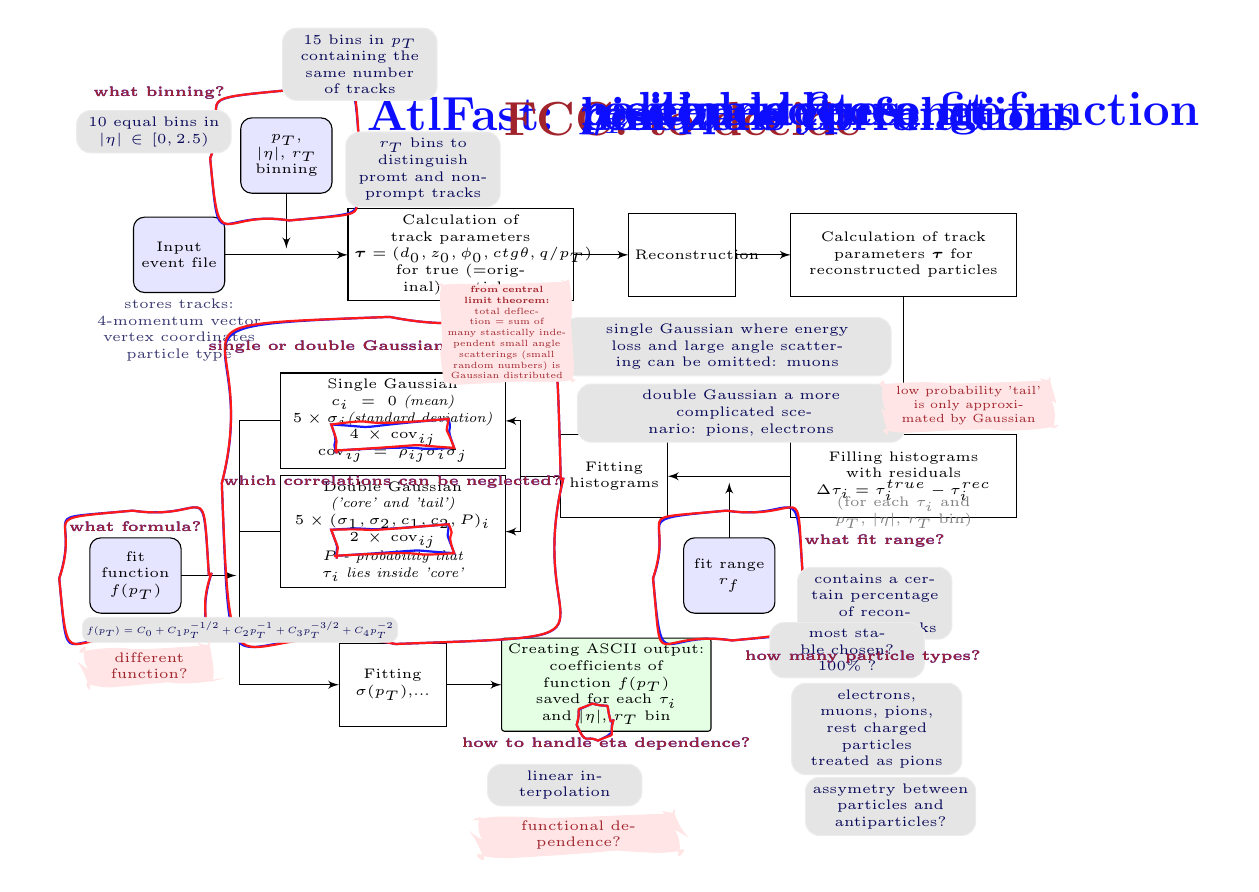
\begin{tikzpicture}[node distance = 20pt, outer sep = 0pt, decoration=penciline]
    tikzstyle{every node}=[font=\tiny]
    \onslide<1->
    {
      \node[input] (inputEV) at (1.,0.) {Input event file};
      \node[comment, below = of inputEV, yshift=20pt, align=center] (inputEVCom) {stores tracks:\\ 4-momentum vector \\ vertex coordinates \\ particle type};
      \node[dot, right = of inputEV] (I1) {};
    }\onslide<3->
    {
      \node[description, right = of I1] (true) {Calculation of track parameters\\ ${\boldsymbol{\tau} = (d_0, z_0, \phi_0, ctg\theta, q/p_T)}$ \\ for true (=original) particles};
    }\onslide<2->
    {
      \node[input, above = of I1, align=center] (Ibins) {$p_T$, $\left|\eta\right|$, $r_T$ \\ binning};
      \draw[arr] (inputEV) --  (true);
      \draw[arr] (Ibins) -- (I1);
    }\onslide<4->
    {
      \node[process, right = of true] (reconstruct) {Reconstruction};
      \draw[arr] (true) --  (reconstruct);
    }\onslide<5->
    {
      \node[description, right = of reconstruct] (reco) {Calculation of track parameters $\boldsymbol{\tau}$ for reconstructed particles};
      \draw[arr] (reconstruct) --  (reco);
    }\onslide<6->
    {
      \node[description, below = of reco, yshift = -30pt] (hist) {Filling histograms with residuals\\ ${\Delta\tau_i = \tau_i^{true} - \tau_i^{rec}  }$ };
      \node[dot, left = of hist] (I2) {};
      \draw[arr] (reco) --  (hist);
    }\onslide<7->
    {
    \node[showComment, below = of hist, yshift = 30pt, text width = 2.8cm] (yell) {(for each $\tau_i$ and $p_T$, $\left|\eta\right|$, $r_T$ bin)};
    }\onslide<9->
    {
      \node[process, left = of I2] (fit) {Fitting histograms};
      \node[dot, left = of fit , xshift=10pt] (I3) {};
    }\onslide<8->
    {
      \node[input, below = of I2, align=center] (Ifit) {fit range $r_f$};
      \draw[arr] (Ifit) --  (I2);
      \draw[arr] (hist) --  (fit);
      %\node[test, below = of Ifit, yshift = 22pt, xshift=-10pt] (yell2) {e.g. given percentage of \\reconstructed tracks in $\pm r_f$};
    }\onslide<10->
    {
      \node[description, left = of fit, yshift= 20pt] (Gauss1) {Single Gaussian\\ {\it $c_i=0$ (mean)\\ $5\times\sigma_i$(standard deviation)\\ $4\times\mathrm{cov}_{ij}$\\ $\mathrm{cov}_{ij}=\rho_{ij}\sigma_i\sigma_j$}};
      \node[dot, left = of Gauss1, yshift= -20pt, xshift = 10pt] (I4) {};
      \draw[line] (fit.west) |- (I3.west);
      \draw[arr]  (I3.west) |- (Gauss1);
    % }\onslide<10-11>
    % {
    %   \node[comment, below = of Gauss1, yshift=-80pt, xshift=-50pt ] (rho) {$\rho_{ij}=\rho(\tau_i\tau_j) = \frac
    %     { \sum_{k=1}^N (\tau_i^{true}-\tau_i^{rec})_k(\tau_j^{true}-\tau_j^{rec})_k }
    %     {}
    %     $};
    }\onslide<11->
    {
      \node[description , left = of fit, yshift= -20pt] (Gauss2) {Double Gaussian {\it('core' and 'tail')\\ $5\times(\sigma_{1},\sigma_{2},c_1,c_2,P)_{i}$\\ $2\times\mathrm{cov}_{ij}$\\ $P$ - probability that $\tau_i$ lies inside 'core'}};
      \draw[arr] (I3.west) |-  (Gauss2);  
    }\onslide<12->
    {
      % \node[output , left = of I4, xshift = 10pt] (eta) {dependence on \\$\left|\eta\right|$ and $r_T$ \\(value/bin)};
      % \draw[arr] (I4)  -- (eta) ;
      \draw[line] (Gauss1)  -| (I4.west) ;
      \draw[line] (Gauss2)  -| (I4.west) ;
    }\onslide<13->
    {
      \node[process , below = of Gauss2] (fitpT) {Fitting $\sigma(p_T)$,...};
    }\onslide<12->
    {
      \node[input , below = of I4,  xshift = -40pt] (IfitpT) {fit function\\ $f(p_T)$};
      \node[dot, below = of I4, right = of  IfitpT] (I5) {};
      \draw[arr] (IfitpT)  -- (I5);
      \draw[arr] (I4.west)  |- (fitpT);
    }\onslide<14->
    {
      \node[outputFILE , right = of fitpT] (ASCII) {Creating ASCII output:\\ coefficients of function $f(p_T)$\\ saved for each $\tau_i$ and $\left|\eta\right|$, $r_T$ bin };
      \draw[arr] (fitpT)  -- (ASCII);
    }\onslide<15-37>
    {
      \node[title1, above = of true, yshift=6pt]  (Prob1Atl) {\LARGE \bf AtlFast:};
    }\onslide<38>
    {
      \node[title2, above = of reconstruct, yshift=6pt]  (Prob1FCC) {\LARGE \bf FCC: to decide};
    }\onslide<16-19>
    {
      \node[Mark1, fit = (Ibins)]  (Pbins) {};
      \node[title1, left = of Pbins.north]  (Pbins1) {\bf what binning?};
      \node[title1, right = of Prob1Atl, xshift=-15pt, yshift=0pt]  (Prob1sub1) {\LARGE \bf bins};
    }\onslide<38>
    {
      \node[title2, left = of Pbins.north]  (Pbins1) {\bf what binning?};
      \node[Mark2, fit = (Ibins)]  (Pbins) {};
    }\onslide<17-19>
    {
      \node[title1ATL, left = of Ibins.north, yshift=-5pt]  (PbinsetaATL) {10 equal bins in \\ $\left|\eta\right|\in [0,2.5)$ };
    }\onslide<18-19>
    {
      \node[title1ATL, above = of Pbins.east]  (PbinsptATL) {15 bins in $p_T$ \\ containing the same number of tracks};
    }\onslide<19>
    {
      \node[title1ATL, right = of Ibins, xshift=-15pt, yshift=-5pt]  (PbinsrtATL) {$r_T$ bins to \\distinguish promt and non-prompt tracks};
    }\onslide<20-22>
    {
      \node[Mark1, fit = (Ifit)]  (Pfit) {};
      \node[title1, right = of Pfit.north, yshift = -10 pt, xshift = 5 pt]  (Pfit1) {\bf what fit range?};
      \node[title1, right = of Prob1Atl, xshift=-15pt]  (Prob1sub1) {\LARGE \bf residuals fit range};
      }\onslide<38>
    {
      \node[Mark2, fit = (Ifit)]  (Pfit) {};
      \node[title2, right = of Pfit.north, yshift = -10 pt, xshift = 5 pt]  (Pfit1) {\bf what fit range?};
    }\onslide<21-22>
    {
      \node[title1ATL, below = of Pfit1, yshift=15pt]  (PfitATL) { contains a certain percentage of reconstructed tracks};
    }\onslide<22>
    {
      \node[title1ATL, below = of PfitATL.north,  xshift=-10pt]  (PfitATL2) {most stable chosen? \\100\% ?};
    }\onslide<23-27>
    {
      \node[Mark1, fit = (Gauss1) (Gauss2)]  (PGauss) {};
      \node[title1, above = of Gauss1, yshift = -15 pt, xshift=-22pt]  (PGauss1) {\bf single or double Gaussian?};
    }\onslide<38>
    {
      \node[Mark2, fit = (Gauss1) (Gauss2)]  (PGauss) {};
      \node[title2, above = of Gauss1, yshift = -15 pt, xshift=-22pt]  (PGauss1) {\bf single or double Gaussian?};
    }\onslide<23-27>
    {
      \node[title1, right = of Prob1Atl, xshift=-15pt]  (Prob1sub1) {\LARGE \bf residuals fit function};
    }\onslide<24-27>
    {
      \node[title1ATLlong, right = of PGauss1, yshift=0pt, xshift=17pt]  (PGaussATL1) {single Gaussian where energy loss and large angle scattering can be omitted: muons};
    }\onslide<25-27>
    {
      \node[title1ATLlong, below = of PGaussATL1, yshift=17pt, xshift=5pt]  (PGaussATL2) {double Gaussian a more\\\ complicated scenario: pions, electrons};
    }\onslide<26-27>
    {
      \scalebox{0.65}{\node[title2ATL, left = of PGaussATL1,  yshift = -10pt , xshift=115pt]  (PGaussATL3) {{\bf from central limit theorem:} \\total deflection = sum of\\ many stastically independent  small angle scatterings (small random numbers) is Gaussian distributed};}
    }\onslide<27>
    {
      \scalebox{0.85}{\node[title2ATL, right = of PGaussATL2,  yshift = -7pt , xshift=22pt]  (PGaussATL4) {low probability 'tail' is only approximated by Gaussian};}
    }\onslide<28>
    {
      \node[Mark1, rectangle,below = of Gauss1, yshift  = 37 pt] (Pcov) {\phantom{~~$4\times\mathrm{cov}_{ij}$~~}};
      \node[Mark1, rectangle,below = of Gauss2, yshift  = 42 pt] (PcovSecond) {\phantom{~~$2\times\mathrm{cov}_{ij}$~~}};
      \node[title1, below = of Pcov, yshift = 13 pt]  (Pcov1) {\bf which correlations can be neglected?};
      \node[title1, right = of Prob1Atl, xshift=-15pt]  (Prob1sub1) {\LARGE \bf non-zero correlations};
    }\onslide<38>
    {
      \node[Mark2, rectangle,below = of Gauss1, yshift  = 37 pt] (Pcov) {\phantom{~~$4\times\mathrm{cov}_{ij}$~~}};
      \node[Mark2, rectangle,below = of Gauss2, yshift  = 42 pt] (PcovSecond) {\phantom{~~$2\times\mathrm{cov}_{ij}$~~}};
      \node[title2, below = of Pcov, yshift = 13 pt]  (Pcov1) {\bf which correlations can be neglected?};
    }\onslide<29-31>
    {
      \node[Mark1, fit = (IfitpT)]  (PfitpT) {};
      \node[title1, above = of IfitpT, yshift = -20 pt, xshift=0pt]  (PfitpT1) {\bf what formula?};
      \node[title1,right = of Prob1Atl, xshift=-15pt]  (Prob1sub1) {\LARGE \bf $p_T$ dependence fit function};
    }\onslide<38>
    {
      \node[Mark2, fit = (IfitpT)]  (PfitpT) {};
      \node[title2, above = of IfitpT, yshift = -20 pt, xshift=0pt]  (PfitpT1) {\bf what formula?};
    }\onslide<30-31>
    {
      \scalebox{0.65}{\node[title1ATLlong, below = of IfitpT, yshift=-52pt, xshift=65pt, text width=6cm]  (PfitpTATL1) {$f(p_T)= C_0 + C_1 p_T^{-1/2} +C_2 p_T^{-1} +C_3 p_T^{-3/2} +C_4 p_T^{-2}$};}
    }\onslide<31>
    {
      \node[title2ATL, below = of IfitpT, yshift=8pt, xshift=5pt, text width=1.5cm]  (PfitpTATL2) {different function?};
    }\onslide<32-34>
    {
      \node[Mark1,circle,below = of ASCII, yshift  = 29 pt, xshift=-4pt] (Peta) {\phantom{$\eta$}};
      \node[title1, below = of ASCII, yshift = 20 pt, xshift=0pt]  (Peta1) {\bf how to handle eta dependence?};
      \node[title1,right = of Prob1Atl, xshift=-15pt]  (Prob1sub1) {\LARGE \bf $\eta$ dependence};
    }\onslide<38>
    {
      \node[Mark2,circle,below = of ASCII, yshift  = 29 pt, xshift=-4pt] (Peta) {\phantom{$\eta$}};
      \node[title2, below = of ASCII, yshift = 20 pt, xshift=0pt]  (Peta1) {\bf how to handle eta dependence?};
    }\onslide<33-34>
    {
      \node[title1ATL, below = of Peta1, yshift=17pt, xshift=-15pt]  (PetaATL1) {linear interpolation};
    }\onslide<34>
    {
      \node[title2ATL, below = of PetaATL1, yshift=17pt, xshift=5pt]  (PetaATL2) {functional dependence?};
    }
    \onslide<35-37>
    {
      \node[title1, right = of ASCII, yshift = 10 pt, xshift=-10pt]  (Ppart) {\bf how many particle types?};
      \node[title1,right = of Prob1Atl, xshift=-15pt]  (Prob1sub1) {\LARGE \bf particle types};
    }
    \onslide<38>
    {
      \node[title2, right = of ASCII, yshift = 10 pt, xshift=-10pt]  (Ppart) {\bf how many particle types?};
    }\onslide<36-37>
    {
      \node[title1ATL, below = of Ppart, yshift=15pt, xshift=5pt, text width = 2cm]  (PpartATL1) {electrons, muons, pions,\\ rest charged particles\\treated as pions};
    }\onslide<37>
    {
      \node[title1ATL, below = of PpartATL1, yshift=19pt, xshift=5pt, text width = 2cm]  (PpartATL2) {assymetry between \\particles and antiparticles?};
    }
\end{tikzpicture}
% \begin{tikzpicture}[overlay,node distance = 20pt, outer sep = 0pt]
%     tikzstyle{every node}=[font=\tiny]
%       \node[title1ATL, left = of Ibins.north, yshift=-5pt, xshift=-5pt]  (Pbinseta) {equal in $\left|\eta\right|$ };
%       \node[title1ATL, below = of Pbinseta, yshift=20pt, xshift=-10pt]  (PbinsetaATL) {10 bins in $\left|\eta\right|\in [0,2.5)$ };

% \end{tikzpicture}

\end{frame}


\begin{frame}
  \begin{center}
    {\textcolor{violet}{\LARGE{\bf Atlfast input data file structure}}}
  \end{center}
\end{frame}

\begin{frame}
\begin{center}
\vskip-10pt
  \includegraphics[height=1.1\textheight]{DataFile}
\begin{tikzpicture}[overlay]
\node[outputFILE] at (1.5,9) {example of\\ ASCII output};
\end{tikzpicture}
\end{center}
\end{frame}


\begin{frame}
  \begin{center}
    {\textcolor{violet}{\LARGE{\bf More on residuals' fitting}}}
  \end{center}
\end{frame}

%% DODAC INFO O TYM JAK SIE DOKLADNIE OBLICZA PARAMETRY - SIGMA, COV, P, etc
\newgeometry{margin=0.1cm}

\begin{frame}{Fitting residuals : $\Delta d_0$, $\Delta z_0$, $\Delta \phi_0$, $\Delta$cot$\theta$,$\Delta q/p_T$ ($\Delta\tau$)}
\begin{columns}
\column{0.45\textwidth}
\hskip-0.3cm
\textcolor{violet}{\Large Single Gaussian}


\includegraphics[width=0.5\textwidth]{Thesis_6_3_part}
\vskip-7pt
\scalebox{0.5}{CERN-THESIS-2004-051 Fig.~6.3.}




\column{0.42\textwidth}
\hskip-0.3cm
\textcolor{violet}{\Large Double Gaussian}


\includegraphics[width=0.5\textwidth]{Thesis_6_10_part}
\vskip-7pt
\scalebox{0.5}{CERN-THESIS-2004-051 Fig.~6.10.}


% $$
% F(\Delta\tau)  =  \frac{f_1}{\sqrt{2\pi} }
% $$



\end{columns}
\end{frame}


\restoregeometry


\begin{frame}
  \begin{center}
    {\textcolor{violet}{\LARGE{\bf Smearing algorithm - Atlfast implementation}}}
  \end{center}
\end{frame}

\begin{frame}%{\bf Schematic picture of handling input data}
\vskip-12pt
  \hskip-1cm
  \begin{tikzpicture}[node distance = 0pt, outer sep = 0pt]
    tikzstyle{every node}=[font=\tiny]
    \onslide<1->
    {
      \node[input] (inputEV) at (7.2,0.4) {Input event file};
      \node[commentDetailed, left = of inputEV, align=center] (inputEVCom) {stores tracks:\\ 4-momentum vector \\ vertex coordinates \\ particle type};
    }\onslide<2->
    {
      \node[className] (smearer) at (7.2,-1.) {TrackSmearer};
      \node[left = of smearer, xshift=-15pt] (sLEFT) {};
      \draw[arr] (inputEV) --  (smearer);
    }\onslide<2>
    {
      \node[comment, right = of smearer] (smearerCom) {called for each track};
    }\onslide<3->
    {
      \node[class, below = of smearer] (ssmear) {::Smear(Track\&)};
    }\onslide<3-7>
    {
      \node[comment, right = of ssmear] (ssmearCom) {Smears track variables\\ $\widetilde{\tau_i}=\tau_i+\rho_i$};
    }
    \onslide<4->
    {
      \node[input] (input) at (-0.5,0) {Input data file};
      \node[commentDetailed, below = of input, align=center] (inputCom) {$\eta_{min}, N_\eta, $\\$C_{0,d_0}$, ...,  \\$C_{0,\rho(d_0,\phi_0)}$,...};
    }\onslide<5->
    {
      \node[className] (manager) at (2,0) {MuonMatrixManager};
      \draw[arr] (input) --  (manager);
      \node[class, below = of manager] (minit) {::initialise()};
      \node[left = of minit, xshift=-15pt] (mLEFT) {};
    }\onslide<5-6>
    {
      \node[comment, right = of minit] (minitCom) {reads file, saves into \\MuonBinData objects};
    }\onslide<6->
    {
      \node[className] (bin) at (2,-4.3) {MuonBinData};
      \draw[arr] (minit.west) -| (mLEFT.east) |- (bin.west);
    }\onslide<6>
    {     \node[comment, right = of bin] (binCom) {stores coefficients for $\eta$ and $r_T$ bins};
    }
    \onslide<7->
    {
      \node[class, below = of minit] (mget) {::getVariables(TrackTrajectory\& track, \\CLHEP::HepSymMatrix\& sigma)};
      \draw[arr] (ssmear.west) -| (sLEFT.south) |-  (mget.east);
    }\onslide<7>
    {
      \node[comment, right = of mget] (mgetCom) {returns vector $\mathbf{\rho}$\\of 5 parameters};
    }
    \onslide<8->
    {
      \node[class, below = of mget] (mgetBinData) {::getBinData(Track\&)};
      \node[left = of mgetBinData, xshift=-5pt] (m2LEFT) {};
      \draw[arr] (mget.west) -| (m2LEFT.east) |- (mgetBinData.west);
    }\onslide<8>
    {
      \node[comment, right = of mgetBinData] (mgetBinDataCom) {returns MuonBinData \\for track's $\eta$ and $r_T$};
    }\onslide<9->
    {
      \node[class, below = of bin] (bgetMatrix) {::getMatrix(Track\&)};
      \node[left = of mget, xshift=-10pt] (m3LEFT) {};
      \draw[arr] (mget.west) -| (m3LEFT.east) |- (bgetMatrix.west);
    }\onslide<9-17>
    {
      \node[comment, right = of bgetMatrix] (bgetMatrixCom) {returns covariance matrix $\mathbf{S}$};
    }\onslide<10->
    {
      \node[className] (params) at (2.,-7) {ParameterResolution};
      \node[class, below = of params] (pres) {::resolution(Track\&)};
      \node[left = of pres, xshift=-5pt] (pLEFT) {};
    }\onslide<10-14,18->
    {
      \draw[arr] (bgetMatrix.west) -| (pLEFT.east) |- (pres.west);
    }\onslide<15-17>
    {
      \draw[->,black!20] (bgetMatrix.west) -| (pLEFT.east) |- (pres.west);
    }\onslide<10>
    {
      \node[comment, right = of pres] (presCom) {calculates $\sigma_{i}$ and $\rho_{ij}$\\ from coefficients $C_k$ \\ ($i,j=d_0,z_0,...$, $k=0,...,4$)};
    }\onslide<12-14>
    {
      \node[commentDetailed, right=of presCom, yshift=10pt] (presComCom) {slope = $\frac{C_{k,\eta_{high}}-C_{k,\eta_{low}}}{\eta_{high}-\eta_{low}}$};
    } \onslide<13-14>
    {
      \node[commentDetailed, below=of presComCom] (presComCom2) { $C_k = C_{k,\eta_{low}}+ slope\times(\eta-\eta_{low})$};
    }\onslide<14-17>
    {
      \node[commentDetailed, below=of presComCom2] (presComCom2) { $\sigma_i$ or $\rho_{ij}$ $= C_0 + C_1 p_T^{-1/2} +C_2 p_T^{-1} +C_3 p_T^{-3/2} +C_4 p_T^{-2}$};
    }\onslide<11-14>
    {
      \node[commentDetailed, above=of presComCom] (presPlot) {\includegraphics[width=0.25\textwidth]{plot}};
    }\onslide<11-13>
    {
      \node[comment, right = of pres] (presCom2) {linear interpolation \\for $\eta$ dependence};
    }\onslide<14>
    {
      \node[comment, right = of pres] (presCom2) {functional \\ $p_{T}$ dependence};
    }\onslide<15>
    {
      \node[commentDetailed, below = of bgetMatrix, align=center] (diagonalsMatrix) {
        $\left[\begin{matrix}
            \sigma_{d_0}^2 & . & . & . & . \\
            . & \sigma_{z_0}^2 & . & . & . \\
            . & . &  \sigma_{\phi_0}^2 &  . & . \\
            . & . & . & \sigma_{ctg\theta}^2 & . \\
            . & . & . & . & \sigma_{q/p_T}^2 \\
          \end{matrix}\right]$
      };
    } \onslide<16>
    {
      \node[commentDetailed, below = of bgetMatrix, align=center] (offdiagonalsMatrix) {
        $\left[\begin{matrix}
            . & . & \rho_{13}{\sigma_{1}\sigma_{3}} & . & \rho_{15}{\sigma_{1}\sigma_{5}}  \\
            . & . & . & \rho_{24}{\sigma_{2}\sigma_{4}}  & . \\
            . & . &  . &  . & \rho_{35}{\sigma_{3}\sigma_{5}}  \\
            . & . & . & . & . \\
            . & . & . & . & . \\
          \end{matrix}\right]$ \\
        additional checks:\\
        if square root $\mathbf{R}$ ($\mathbf{RR}=\mathbf{S}$) exists\\
        and if $\rho_{ij}\in[-1,1]$
      };

    }\onslide<17>
    {
      \node[commentDetailed, below = of bgetMatrix, align=center] (allMatrix) {
        $\left[\begin{matrix}
            \sigma_{1}^2 & . & \rho_{13}{\sigma_{1}\sigma_{3}} & . & \rho_{15}{\sigma_{1}\sigma_{5}}  \\
            . & \sigma_{2}^2 & . &  & \rho_{24}{\sigma_{2}\sigma_{4}}  & . \\
            \rho_{13}{\sigma_{1}\sigma_{3}} & . &  \sigma_{3}^2 &  . & \rho_{35}{\sigma_{3}\sigma_{5}}  \\
            . & \rho_{24}{\sigma_{2}\sigma_{4}} & . & \sigma_{4}^2 & . \\
            \rho_{15}{\sigma_{1}\sigma_{5}} & . & \rho_{35}{\sigma_{3}\sigma_{5}} & . & \sigma_{5}^2 \\
          \end{matrix}\right]$ 
      };

    } \onslide<18->
    {
      \node[className] (corr) at (6.,-2) {CorrelatedData};
      \node[class, below = of corr] (cgen) {::generate(CLHEP::HepMatrix\&)};
      \node[left = of mget, yshift=-20pt, xshift=-7.5pt] (mDOWN) {};
      \draw[arr] (mget.west) -| (mDOWN.east) |- (cgen.west);

    } \onslide<19-22>
    {
      \node[comment, right = of cgen] (cgenCom) {returns the result of $\mathbf{R} \times \mathbf{N}$};
    } \onslide<20->
    {

      \node[class, below = of cgen ] (croot) {::root(CLHEP::HepMatrix\&)};
      \node[left = of croot, xshift=-10pt] (c2LEFT) {};
      \draw[arr] (cgen.west)  -| (c2LEFT.east) |- (croot.west);
    } \onslide<20>
    {

      \node[comment, right = of croot] (crootCom) {calculates matrix $\mathbf{R}$, a square root of matrix $\mathbf{S}$ ($\mathbf{R}\mathbf{R}=\mathbf{S}$),  implementation of Cholesky decomposition};
    }\onslide<21>
    {
      \node[commentDetailed, below = of croot, align=center] (rootMatrix) {
        \scalebox{0.6}
        {
         $ \mathbf{S} =  \left[\begin{matrix}

            \sigma_{1} &  & &  &  \\

            0 & \sigma_{2} &  &   & &  \\

            \rho_{13}{\sigma_{3}} & 0 &  \sigma_{3}\sqrt{1-\rho_{13}\frac{\sigma_{1}}{\sigma_{3}}} &   & \\

            0 & \rho_{24}\sigma_{4} & 0 & \sigma_{4}\sqrt{1-\rho_{24}\frac{\sigma_{2}}{\sigma_{4}}} &  \\

            \rho_{15}\sigma_{5} & 0 & \frac{\sigma_5(\rho_{35}-\rho_{13}\rho_{15})} { 1 - \rho_{13}\frac{\sigma_{1}}{\sigma_{3}}} & . & \sigma_{5}\sqrt{1-\rho_{15}\frac{\sigma_1}{\sigma_5}-\rho_{35}\frac{\sigma_3}{\sigma_5}} \\

          \end{matrix}\right]  \left[\begin{matrix}

            \sigma_{1} & 0 & \rho_{13}\sigma_{3} & 0 & \rho_{15}\sigma_{5}  \\

             & \sigma_{2} & 0 &   & \rho_{24}\sigma_{4}  & 0 \\

            &  &  \sigma_{3}\sqrt{1-\rho_{13}\frac{\sigma_{1}}{\sigma_{3}}} &  0 & \frac{\sigma_5(\rho_{35}-\rho_{13}\rho_{15})} { 1 - \rho_{13}\frac{\sigma_{1}}{\sigma_{3}}} \\

            &  &  & \sigma_{4}\sqrt{1-\rho_{24}\frac{\sigma_{2}}{\sigma_{4}}} & 0 \\

            &  &  & & \sigma_{5}\sqrt{1-\rho_{15}\frac{\sigma_1}{\sigma_5}-\rho_{35}\frac{\sigma_3}{\sigma_5}} \\

          \end{matrix}\right]$
        }
      };

    } \onslide<22->
    {
      \node[class, below = of croot] (cnorm) {::normal(int)};
      \node[left = of cnorm, xshift=-5pt] (cLEFT) {};
      \draw[arr] (cgen.west) -| (cLEFT.east) |- (cnorm.west);
    } \onslide<22-23>
    {
      \node[comment, right = of cnorm] (cnormCom) {generates vector $\mathbf{N}$ (of 5 numbers from normal distribution)};
    } \onslide<23->
    { \node[class, below = of cnorm] (cdev) {:::makeDeviate\\(pair$<$double,double$>$,\\ double\&)};
      \draw[arr] (cdev.west)  -| (cLEFT.east) |- (cdev.west);
    } \onslide<23>
    {
      \node[comment, right = of cdev] (cdevCom) {impelementation of Fast Normal Random Number Generator \\(ALG 712 J.L.Leva)};
    }
    \onslide<24>{}


% \draw[->,redish, thick] (pres.west)  edge [bend left] node[rotate=90, yshift=5pt] {$\sigma_{i}$, $\rho_{ij}$, }  (bgetMatrix.west);
  \end{tikzpicture}
\end{frame}

\begin{frame}
  \begin{center}
    {\textcolor{violet}{\LARGE{\bf Validation}}}
  \end{center}
\end{frame}

\newgeometry{margin=1cm}

\begin{frame}
\small{
\color{violet}{\large \bf Tools:}
\begin{itemize}
\item plots of residuals: $d_0^{true}-d_0^{rec}$, $z_0^{true}-z_0^{rec}$, $\phi_0^{true}-\phi_0^{rec}$, $ctg\theta^{true}-ctg\theta^{rec}$ and $q/p_T^{true}-q/p_T^{rec}$;
\item plots of correlations: $\rho_{d_0,z_0}^{rec} (\rho_{d_0,z_0}^{tru})$, etc.;
\item $\chi^2$ test:
  $$
    \chi^2_{\tau_i}=\sum_{bins}\frac{\Delta\tau_i^{fast}-\Delta\tau_i^{full}}{\tau_i^{full}}
  $$
\end{itemize}
\vfill
\color{violet}{\large \bf Parametrisation tests:}
\begin{enumerate}
\item Binning in $\left| \eta\right|$, $p_T$ and $r_T$;
\item Fit ranges on residuals' plots;
\item Fit formula to residuals' plots: single/double Gaussian;
\item Decide which correlations are significant;
\item Fit formula to describe $p_T$ dependence;
\item Linear interpolation or functional $\left| \eta\right|$ dependence;
\end{enumerate}
\vfill
\color{violet}{\large \bf Validation:}
\begin{enumerate}
\item Cross-check against the full simulation (and fast with reconstruction) using the same event sample as for parameters' extraction;
\item Cross-check against the full simulation (and fast with reconstruction) using different event sample (H$\rightarrow$ZZ*$\rightarrow 4\mu$ ?);
\end{enumerate}
}
\vfill
\end{frame}
\restoregeometry



\end{document}